Convolution Neural Network (CNN) คือโมเดลปัญญาประดิษฐ์ประเภทหนึ่งมักจะนำมาใช้กับงานที่เกี่ยวกับการจำแนกวัตถุในภาพ เช่น แมว หมา มนุษย์ รถ เป็นต้น
การที่ CNN สามารถจำแนกภาพออกมาได้ว่าเป็นประเภทอะไรนั้นต้องผ่านชั้นตัวกรอง (filter layer) หรือเคอร์เนล (kernel), pooling layer, fully connected layer (FC) 
และใช้ softmax หรือ logistic function ในการจำแนกว่าเป็นวัตถุประเภทอะไร ดังรูปที่ \ref{fig:CNN architecture}

\begin{figure}[!ht]
	\centering
	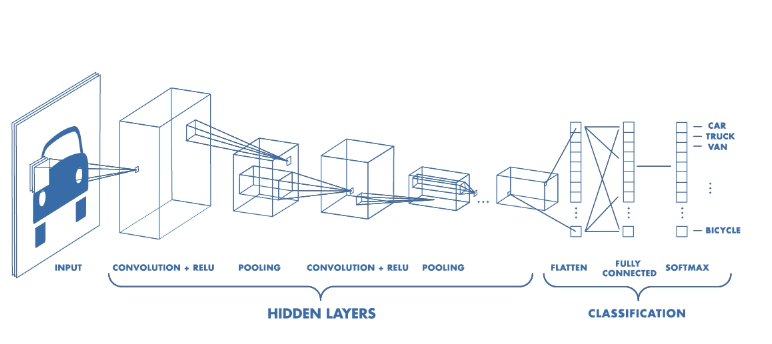
\includegraphics[width=1\textwidth]{chapter2/images/CNN.png}
		\caption{ตัวอย่างโครงสร้างของ CNN ที่ใช้ในการจำแนกประเภทของรูปภาพ}
    	\label{fig:CNN architecture}
\end{figure}

\subsection*{ตัวกรอง/เคอร์เนล (Filter/Kernel)}
ตัวกรองหรือเคอร์เนล คือชั้นที่ใช้ในการสกัดคุณลักษณะของรูปภาพออกมาด้วยสี่เหลี่ยมเล็กๆขนาด NxN โดยที่ N$\in$[1, 2, 3, ...] ดังรูปที่ \ref{fig:kernel_3x3} 
และสมมติให้ภาพที่ใช้ในการประมวลผมเป็นดังรูปที่ \ref{fig:input_ex}
\begin{figure}[!ht]
	\centering
	\begin{subfigure}[b]{0.5\textwidth}
        \centering
        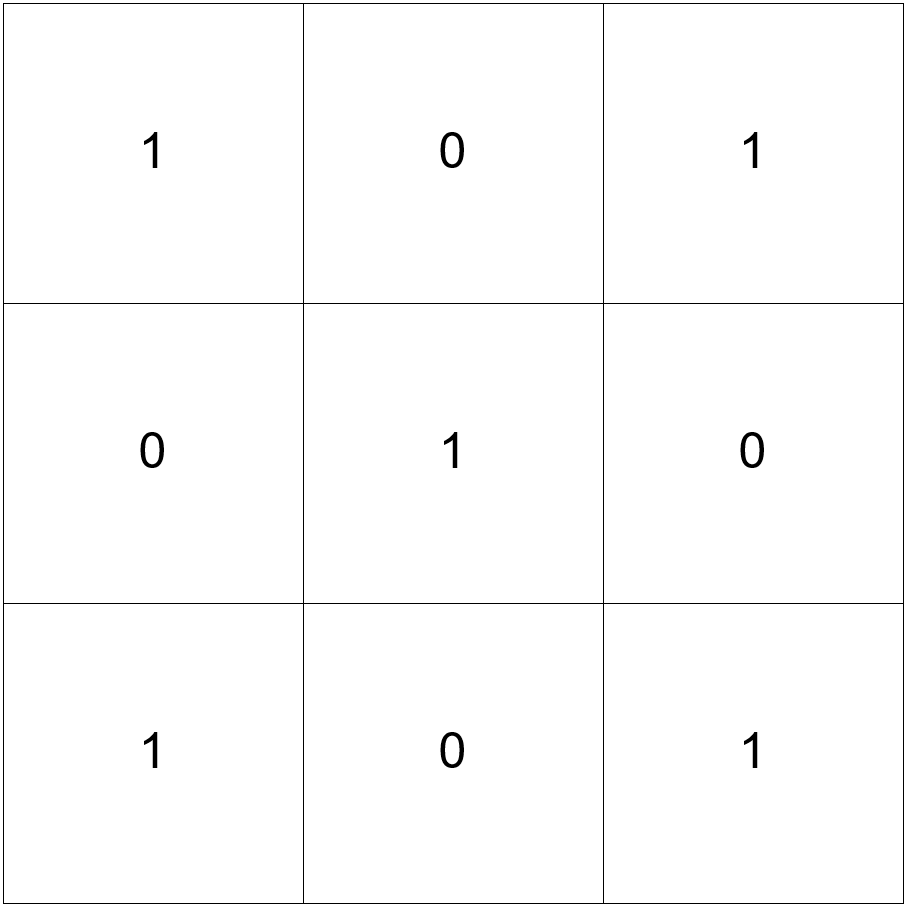
\includegraphics[width=0.4\textwidth]{chapter2/images/kernel_ex.png}
		\caption{ตัวอย่างเคอร์เนลขนาด 3x3}
		\label{fig:kernel_3x3}
    \end{subfigure}
    \begin{subfigure}[b]{0.5\textwidth}
        \centering
		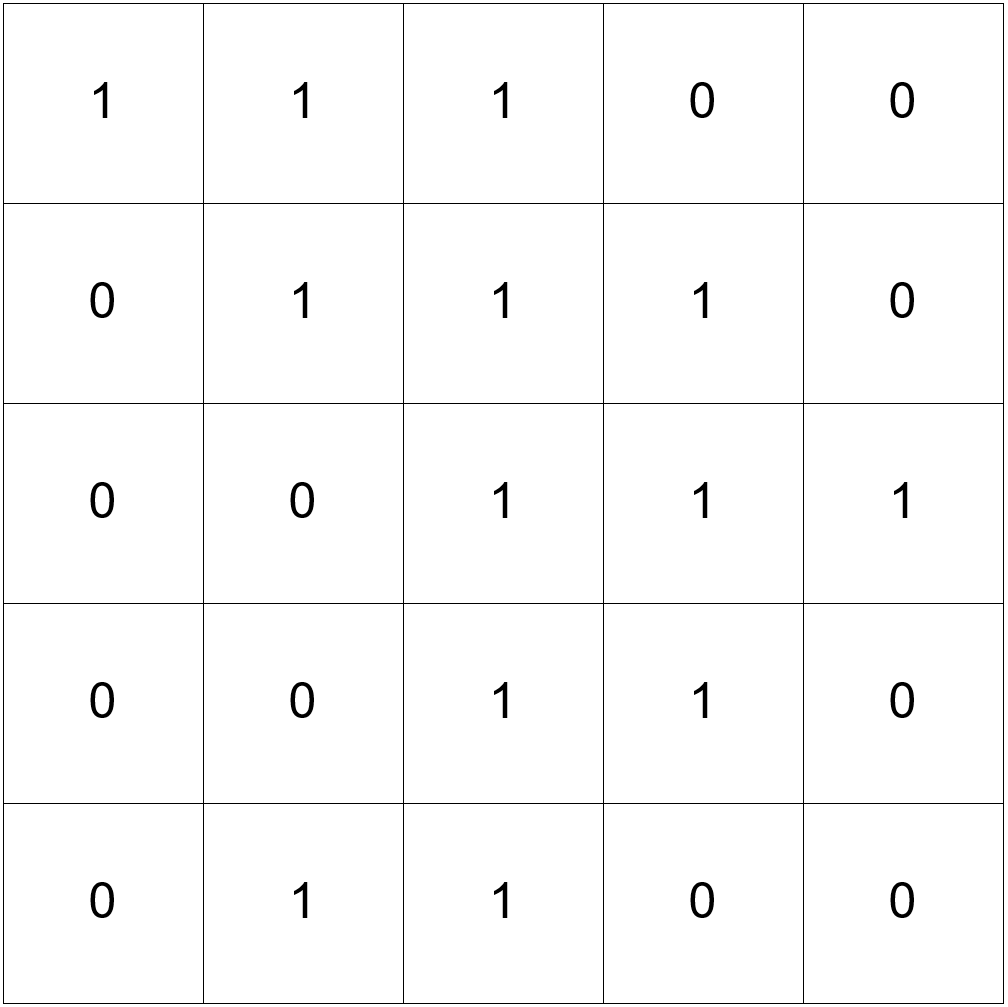
\includegraphics[width=0.5\textwidth]{chapter2/images/input_ex.png}
		\caption{ตัวอย่างภาพที่ใช้ในการประมวลผล}
        \label{fig:input_ex}
	\end{subfigure}
	\caption{ตัวอย่างเคอร์เนล และภาพที่ใช้ในการประมวลผล}
	\label{fig:kernel_input_ex}
\end{figure}
\clearpage
เมื่อนำเคอร์เนล (รูปที่ \ref{fig:kernel_3x3}) ไปทาบกับภาพ (รูปที่ \ref{fig:input_ex}) แล้วคูณค่าในเคอร์เนลกับพิกเซล (pixel) ที่ทาบจะได้คุณลักษณะของช่องนั้นจากนั้นเลื่อนต่อไปจนครบทั้งรูป 
ซึ่งการเลื่อน (Stride) นั้นขึ้นอยู่กับผู้สร้างว่าต้องการจะให้เลื่อนครั้งละกี่ช่อง แต่ระยะการเลื่อนที่มากขึ้นจะทำให้สัมพันธ์ของคุณลักษณะที่ได้ออกมาน้อยลงด้วย โดยการวางเคอร์เนลเทียบบนภาพนั้นจะวางไม่ไห้เกินกรอบรูป 
แต่ถ้าต้องการทาบกับทุกพิกเซลในภาพสามารถทำได้ โดยการให้พื้นที่ที่เกินขอบภาพไปเท่ากับ 0 เทคนิคนี้เรียกว่า padding และคุณลักษณะที่ได้ออกมาทั้งหมดจะเรียกว่าผังคุณลักษณะ (features map) ตามรูปที่ \ref{fig:example feature map}

\begin{figure}[!ht]
	\centering
	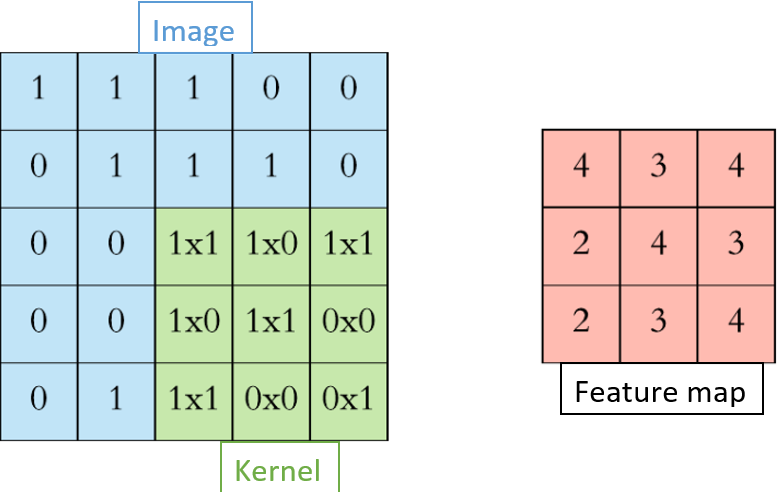
\includegraphics[width=0.5\textwidth]{chapter2/images/feature_map.png}
		\caption{ตัวอย่างการหาผังคุณลักษณะ }
    	\label{fig:example feature map}
\end{figure}

\subsection*{Pooling}
Pooling คือชั้นที่สามารถลดขนาดของภาพลงเพื่อลดข้อมูลที่ไม่จำเป็นลง ซึ่งมีหลายประเภทแต่นิยมใช้มีสองประเภทได้แก่ max pooling และ average pooling
โดยที่ max pooling จะใช้ในการหาค่าที่มากที่สุดในเคอร์เนลที่ทาบอยู่ดังรูปที่ \ref{fig:example max pooling} ในขณะที่ average pooling 
จะหาค่าเฉลี่ยของภายในเคอร์เนลออกมาดังรูปที่ \ref{fig:example average pooling}
\begin{figure}[!ht]
	\centering
	\begin{subfigure}[b]{1.0\textwidth}
		\centering
		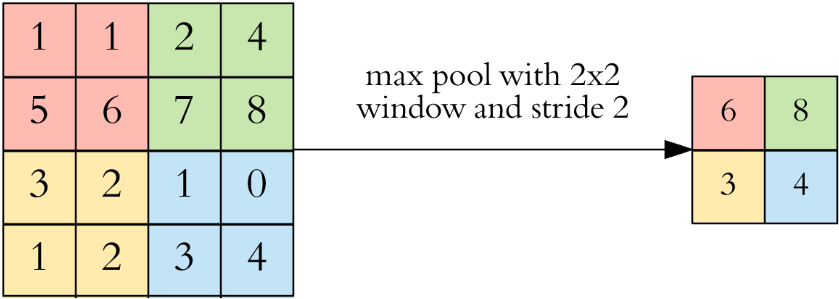
\includegraphics[width=0.5\textwidth]{chapter2/images/max_pooling.png}
		\caption{ตัวอย่างการทำ max pooling}
		\label{fig:example max pooling}
    \end{subfigure}
    \begin{subfigure}[b]{1.0\textwidth}
        \centering
		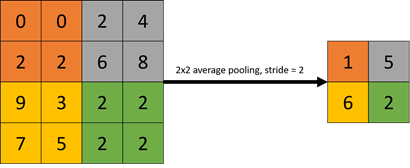
\includegraphics[width=0.5\textwidth]{chapter2/images/average_pooling.png}
		\caption{ตัวอย่างการทำ average pooling}
		\label{fig:example average pooling}
	\end{subfigure}
	\caption{ตัวอย่างการใช้ max pooling และ average pooling กับภาพ}
	\label{fig:pooling_ex}
\end{figure}
\clearpage

\subsection*{Activation function}
ในแต่ละชั้นของ CNN นั้นจะมี activation function เป็นสิ่งที่กำหนดว่าเอาท์พุตของชั้นนั้นว่าจะอยู่ในช่วงไหน 
เช่น -1 ถึง 1, 0 ถึง 1 ขึ้นอยู่กับฟังก์ชั่นที่ใช้ ซึ่งจะแบ่งออกเป็นสองแบบคือ แบบเป็นเส้นตรง และแบบไม่เป็นเส้นตรง

แบบเป็นเส้นตรงจะมีสมการของฟังก์ชั่นดังนี้ $ f(x) = x $ โดยที่ $x$ คืออินพุตของฟังก์ชั่น ทำให้เอาท์พุตที่ได้จากฟังก์ชั่นนี้มีค่าอยู่ในช่วง -inf ถึง inf

แบบไม่เป็นเส้นตรงจะมีหลายฟังก์ชั่น แต่ฟังก์ชั่นที่เป็นที่นิยมใช้คือ Rectified Linear Unit หรือ ReLU, Leaky ReLU และ Parametric ReLU โดยทั้งสามฟังก์ชั่นมีสมการดังนี้\\
\textbf{ReLU}\\
$ f(x) =
\begin{cases}
	0 & \text{if } x < 0,\\
	x & \text{otherwise}
\end{cases}
$\\
\textbf{Leaky ReLU}\\
$ f(x) =
\begin{cases}
	0.01x & \text{if } x < 0,\\
	x & \text{otherwise}
\end{cases}
$\\
\textbf{Parametric ReLU} โดยที่ $\alpha\in\mathbb{R^+}$\\
$ f(x) =
\begin{cases}
	\alpha x & \text{if } x < 0,\\
	x & \text{otherwise}
\end{cases}
$
\subsection*{Fully connected layer}
เป็นชั้นที่จะรวมคุณลักษณะทั้งหมดของชั้นก่อนหน้าเป็นเวกเตอร์ ก่อนที่จะนำเวกเตอร์ที่ได้ไปผ่าน activation function เพื่อคำนวณหาคำตอบสำหรับการแยกประเภทของภาพ
ซึ่งฟังก์ชั่นที่นิยมใช้จะมีสองฟังก์ชั่น คือ softmax และ sigmoid (logistic) โดยทั้งสองมีความแตกต่างกันดังตารางที่
\begin{table}[!ht]
	\centering
	\begin{tabular}{|c|c|c|}
		\hline
		{} & Softmax & Sigmoid\\
		\hline\hline
		1 & \begin{tabular}{@{}c@{}}สมการคือ $f(x_i) = \frac{exp(x_i)}{\sum_{j=0}^k exp(x_j)}$ \\โดยที่ k คือจำนวนข้อมูล และ i$\in${0, 1, 2, ..., k}\end{tabular} & $f(x_i) = \frac{1}{1+exp(-x_i)}$ โดยที่ i$\in${0, 1, 2, ..., k}\\
		\hline
		2 & ผลรวมของความน่าจะเป็นจะเท่ากับ 1 เสมอ & ผลรวมของความน่าจะเป็นไม่จำเป็นต้องเท่ากับ 1\\
		\hline
		3 & มักใช้ในการจำแนกประเภทมากกว่าสองประเภทขึ้นไป & มักใช้ในการจำแนกประเภทเพียงสองประเภท\\
		\hline
	\end{tabular}
	\caption{ตารางแสดงการเปรียบเทียบระหว่าง softmax function และ sigmoid function}
	\label{tab:softmax_vs_sigmoid}
\end{table}
\clearpage
\subsection*{Intersection Over Union (IoU)}
\begin{figure}[!ht]
	\centering
	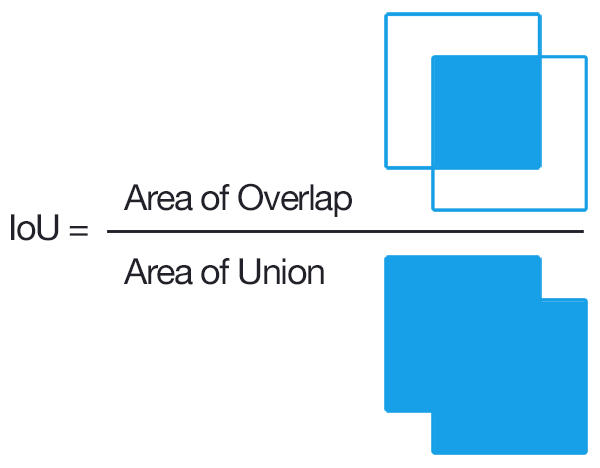
\includegraphics[scale=0.3]{chapter2/images/iou_equation.png}
		\caption{ภาพแสดงการหา IoU ของกรอบสี่เหลี่ยมจริงของเฟรม และ กรอบสี่เหลี่ยมที่ทำนายขึ้นมา}
    	\label{fig:iou_equation}
\end{figure}
เป็นวิธีในการทดสอบประสิทธิภาพของการตรวจจับวัตถุ โดยค่า IoU นั้นสามารถหาได้จากการนำกรอบสี่เหลี่ยมจริงของวัตถุ 
และกรอบสี่เหลี่ยมที่ได้จากการทำนายมาหาอัตราส่วนระหว่างพื้นที่ที่กรอบสี่เหลี่ยมทั้งสองทับซ้อนกัน และหารด้วยพื้นที่ทั้งหมดของกรอบสี่เหลี่ยมทั้งสองรวมกัน ซึ่งสามารถเขียนในรูปสมการได้ดังนี้
\begin{equation}
IoU(P,G) = \frac{\left| P \cap G \right|}{\left| P \cup  G \right|}					
\end{equation}
โดยที่
\begin{conditions}
IoU			&  ค่าที่ใช้สำหรับวัดผลความใกล้เคียงระหว่างสองกรอบสี่เหลี่ยม    \\
P			&  พื้นที่ของกรอบสี่เหลี่ยมที่ทำนายได้	\\
G			&  พื้นที่ของกรอบสี่เหลี่ยมจริงของรูปภาพ					\\
\end{conditions}

\subsection*{Non Maximum Suppression (NMS)}
Non Maximum Suppression คือ อัลกอริทึ่มที่นิยมใช้เข้ามาช่วยจัดการปัญหากรอบสี่เหลี่ยมที่ซ้อนทับกันซึ่งเกิดจากการทำนายซ้ำ เพื่อให้ได้กรอบสี่เหลี่ยมที่บ่งบอกถึงตำแหน่งของวัตถุนั้นเพียงกรอบเดียว 
\begin{figure}[!ht]
	\centering
	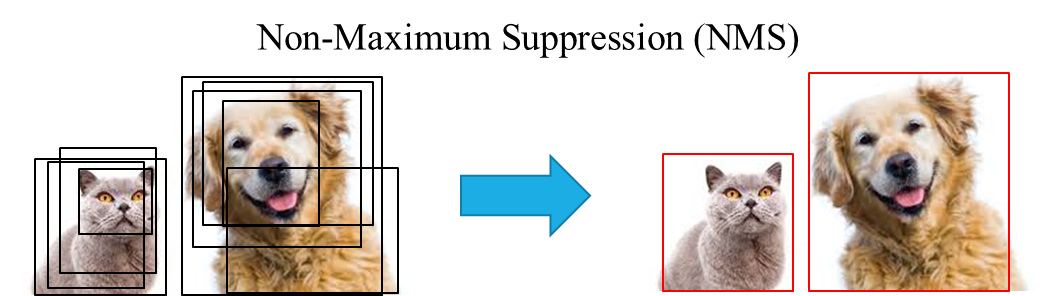
\includegraphics[scale=0.3]{chapter2/images/NMS.png}
		\caption{ตัวอย่างการทำงานของ NMS}
    	\label{fig:NMS}
\end{figure}
